\documentclass[a4paper,11pt,landscape,exos]{nsi} % COMPILE WITH DRAFT
\usepackage{hyperref}

\pagestyle{empty}
\setlength{\columnseprule}{0.5pt}
\setlength{\columnsep}{1cm}
\begin{document}

\begin{multicols}{2}
    \textcolor{UGLiBlue}{NOM, Prénom :\\
    Date : vendredi 16/05/2025}\\
\classe{\premiere spe}
\titre{
\includegraphics[width=3cm]{CAN.png} Interrogation 4}
\maketitle

\begin{enumerate}[itemsep=1em]
    \item  $12-6\times9$
	\item $25\,\%$ de $120$
	\item Écrire sous forme d'une fraction irréductible $\dfrac{9}{4}\times \dfrac{-7}{9}$.
	\item $3^{4}\times 3^{5}=3^{\ldots}$
	\item $2-\dfrac{1}{7}$ 
	\item Soit le script Python : 

\medskip
\medskip\hspace*{10mm}\fbox{\parbox{0.5\linewidth}{\setlength{\parskip}{.5cm} \texttt{def resultat(a) :}\newline \hspace*{7mm}\texttt{return (a**2+3*a)}}}\newline\medskip\\Que renvoie  $\texttt{resultat(2)}$ ?
	\item $A$ et $B$ sont des événements indépendants tels que $P(A)=0{,}1$ et $P(B)=0{,}4$.
\\ $P(A\cap B)=\ldots$.
	\item La suite $(u_n)$ est géométrique telle que  $u_{6}= 10$ et $u_{7}= 5$.\\Sa raison $q$ est $\ldots$
	\item Quel est l'extremum sur $\mathbb{R}$ de  $x\longmapsto -2(x+3)^2+15$ ?  
	\item $\vec{u}\begin{pmatrix}5 \\3\end{pmatrix}$ et $\vec{v}\begin{pmatrix}20 \\ -12\end{pmatrix}$ ont la même direction. \\ 
    
    	$\square\;$ Vrai\qquad $\square\;$ Faux\qquad 
	\item Donner le nombre d'antécédent(s) de $3$ par la fonction carré. 
	\item $425^2-424^2$ 
	\item Deux diminutions successives de  $50\,\%$ correspondent à une diminution globale de  $\ldots \,\%$.
	\item $\pc{A}{-3}{7}$ et $\pc{B}{-2}{-4}$\\[.5em]
         $\vc{AB}{\ldots}{\ldots}$
	\item $A$ et $B$ sont deux événements tels que :
    \begin{center}
        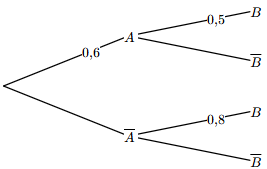
\includegraphics[width=5cm]{Interro4_arbre.png}
    \end{center}$P(B)=\ldots$ 

\end{enumerate}


\vfill\null
\end{multicols}

\newpage

\begin{multicols}{2}
    \classe{\premiere spe}
\titre{
\includegraphics[width=3cm]{CAN.png} Corrigé Interro 4}
\maketitle

\begin{enumerate}[itemsep=1em]
    \item $12-6\times9={\color[HTML]{f15929}\boldsymbol{-42}}$
\item $25\,\%$ de $120 = {\color[HTML]{f15929}\boldsymbol{30}}$\\ Prendre $25\,\%$  de $120$ revient à prendre le quart de $120$.\\
      Ainsi, $25\,\%$ de $120$ est égal à $120\div 4 =30$.
     
\item $\dfrac{9}{4}\times \dfrac{-7}{9}=-\dfrac{7{\color[HTML]{2563a5}\boldsymbol{\times9}} }{4{\color[HTML]{2563a5}\boldsymbol{\times9}}}={\color[HTML]{f15929}\boldsymbol{-\dfrac{7}{4}}}$
\item On utilise la formule $a^n\times a^m=a^{n+m}$ avec $a=3$, $n=4$ et $p=5$.\\
            $3^{4}\times 3^{5}=3^{4+5}=3^{{\color[HTML]{f15929}\boldsymbol{9}}}$
\item On a : \\$\begin{aligned}
      2+\dfrac{1}{7} &= \dfrac{2 \times 7}{7} - \dfrac{1}{7} \\
      &= \dfrac{14}{7} - \dfrac{1}{7}\\
      &  ={\color[HTML]{f15929}\boldsymbol{\dfrac{13}{7}}}
      \end{aligned}$
\item  L'algorithme renvoie $2^2+3\times2={\color[HTML]{f15929}\boldsymbol{10}}$.
\item  Comme $A$ et $B$ sont des événements indépendants,  $P(A\cap B)=P(A)\times  P(B)$.\\
Ainsi, \\
$\begin{aligned}
P(A\cap B)&=0{,}1 \times 0{,}4\\
P(A\cap B)&={\color[HTML]{f15929}\boldsymbol{0{,}04}}
\end{aligned}$
  
\item On passe de $u_{6}$ à $u_{7}$ en divisant par $2$, c'est-à-dire en multipliant par $\dfrac{1}{2}$.\\
    La raison de la suite est donc ${\color[HTML]{f15929}\boldsymbol{\dfrac{1}{2}}}$.
\item On reconnaît la forme canonique d'une fonction polynôme du second degré :\[f(x)=a(x-\alpha)^2+\beta\] où $\beta$ est l'extremum.\\
    L'extremum de $f$ est ${\color[HTML]{f15929}\boldsymbol{15}}$.
\item  
    
    	$\square\;$ Vrai\qquad $\blacksquare\;$ Faux\qquad Les vecteurs ont la même direction lorsqu'ils sont colinéaires.\\
    On a $x_{\vec{v}}=4\times x_{\vec{u}}$ mais $y_{\vec{v}}\neq 4\times y_{\vec{u}}$, donc les vecteurs n'ont pas la même direction.
\item Comme $3 > 0$, l'équation $x^2=3$   a deux solutions . \\
    Ainsi, $3$ a ${\color[HTML]{f15929}\boldsymbol{2}}$ antécédents par la fonction carré.
\item On utilise l'égalité remarquable $a^2-b^2=(a+b)(a-b)$ avec $a=425$ et $b=424$.\\
    $\begin{aligned}
    425^2-424^2&=(425+424)(425-424)\\
    &=849\times 1\\
    &={\color[HTML]{f15929}\boldsymbol{849}}
    \end{aligned}$
\item  Le coefficient multiplicateur  associé à une baisse de $50\,\%$ est $0{,}5$.\\
    Le coefficient multiplicateur global associé à ces deux diminutions est $0{,}5\times 0{,}5= 0{,}25$.\\
    On en déduit que le taux d'évolution globale est $0{,}25-1=-0{,}75$.\\
    La diminution globale est donc de ${\color[HTML]{f15929}\boldsymbol{75}} \,\%$.
\item $\vc{AB}{x_B-x_A}{y_B-y_A}$ donc $\vc{AB}{-2-(-3)}{-4-7}$.\\
         Ainsi, $\vc{AB}{\color[HTML]{f15929}{1}}{\color[HTML]{f15929}{-11}}$.
\item On utilise la formule des probabilités totales pour calculer $P(B)$ :\\
              $\begin{aligned}
              P(B)&=P(A\cap B)+P(\bar{A}\cap B)\\
              &=0{,}6\times 0{,}5+0{,}4\times 0{,}8\\
    &={\color[HTML]{f15929}\boldsymbol{0{,}62}}
              \end{aligned}$
\end{enumerate}
\end{multicols}

\end{document}